In order to remove the drift of the drone, it is necessary to implement an outer feedback loop that controls and corrects the position and velocity. This can be done by using the Optitrack system in Cyberzoo. In this section, the flight plan using the Optitrack system is proposed and discussed. There are two flight plans proposed - one that actively moves the waypoints, and the other which uses a preset fixed waypoints.\\

\subsection{Flight Plan I - Moving Waypoints}
This flight plan simply does the two main things. First, if the drone detects an obstacle nearby, it either turns to the left or right. It performs this maneuver in two steps of $45^o$ to ensure the stable turning of the heading. Secondly, if the drone goes outside the predefined flight area, it turns around and sets the waypoint to the opposite side of the flight area. The turning maneuver is again carried out intermittently in four steps of $45^o$ turns. If the drone neither detects an obstacle nearby or goes out-of-bounds, it simply flies forward with a constant speed. This flight plan logic is illustrated in Figure \ref{fp1}. Note that this flight plan is called "moving waypoints" because the maneuvers like stopping and turning are carried out by actively and continuously relocating the waypoints for the desired flight trajectory.

\begin{figure}[H]
	\centering
	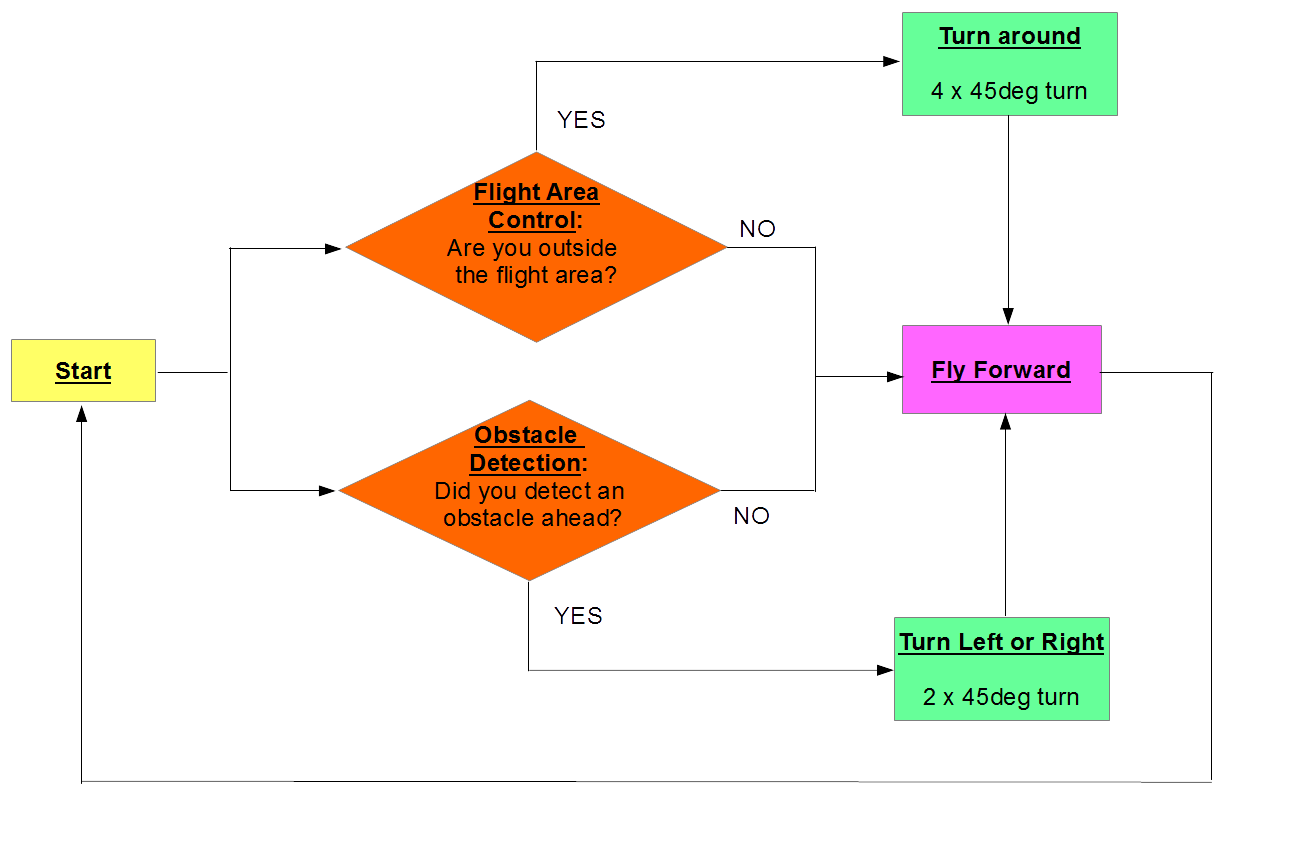
\includegraphics[width = 0.5\textwidth]{Figures/FP1.png}
	\caption{Logic used for the Flight Plan I - Moving Waypoints.}
	\label{fp1}
\end{figure}